
\section{processes.xml}

The process file is used to define constraints related to complex
cellular processes.

\subsection{RBAProcesses}
\label{sec:rba_processes}

The outermost portion of the process file is an instance of class
\rbaprocesses, shown in Figure~\ref{fig:processes_doc}.

\begin{figure}
  \centering
  \includegraphics[scale=0.8]{figures/processes_doc}
  \caption{XML structure of process document.}
\label{fig:processes_doc}
\end{figure}

\rbamacromolecules{} has no simple attributes.
It contains exactly one instance of \textbf{ListOfProcesses}
and \textbf{ListOfComponentMaps}.


\subsection{Process}
\label{sec:process}

The \process{} class is used to define cellular processes
(Fig.~\ref{fig:processes_process}).
Processes cover a wide variety of non-metabolic reactions.

\begin{figure}
  \centering
  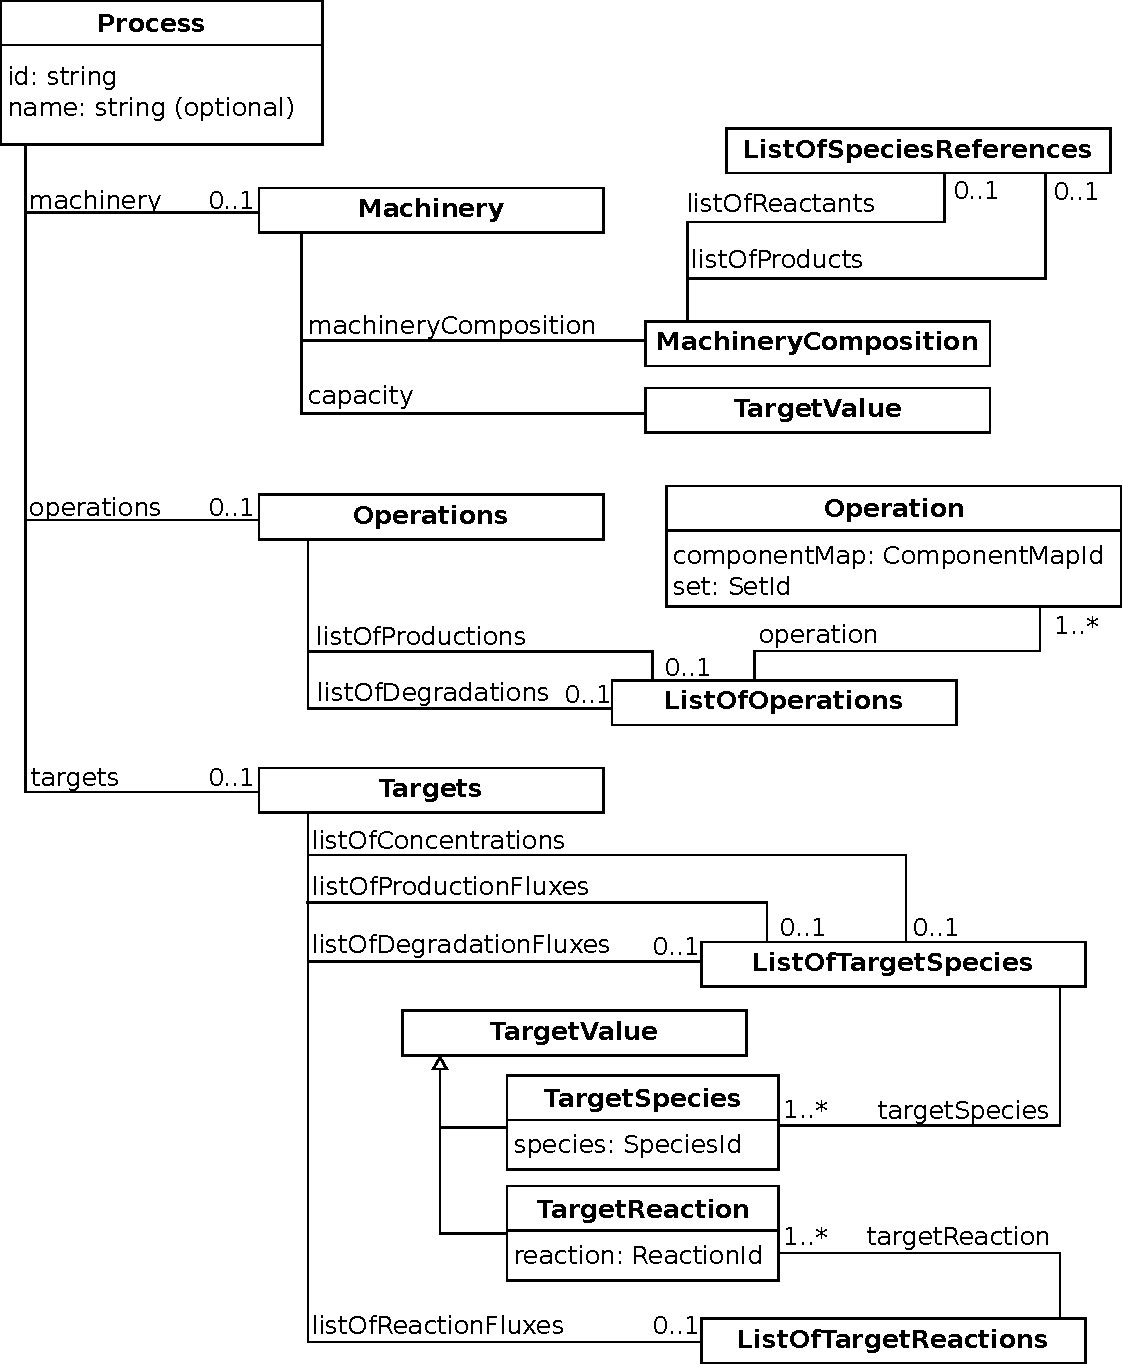
\includegraphics[scale=0.8]{figures/processes_process}
  \caption{Class used to store processes.}
\label{fig:processes_process}
\end{figure}

A \process{} revolves around 3 optional substructures.
We encourage you to study existing examples to understand how the different
substructures are used.

The \machinery{} is the molecular entity enabling the process
(\textit{e.g.} ribosome for translation.)
Each machinery unit has a limited production/degradation capacity.
Every target of a process has an intrinsic metabolite cost
(metabolites needed to produce/degrade it and byproducts).
However, if a machinery is defined, there is an additional metabolic cost
to produce the machinery that will enable the production/degradation of the
target.
This is similar to the production of \enzyme{}s in order to catalyze
metabolic \reaction{}s.

\operations{} define the sets of macromolecules that a process
produces or degrades.
A \macromolecule{} can only be produced if it was related to a \process{}.
For example, a protein can only be produced if there is a translation process
where proteins are explicitly listed as a production in \operations{}.
\operations{} break down \macromolecule{}s in metabolic \species{}
and \machinery{} costs.
\operations{} does not define how many molecules of a \macromolecule{}
must be produced.

\targets{} define the fluxes that a process must maintain for the cell
to work properly.
Some fluxes, such as enzyme production, are already enclosed in the base model.
They should not appear in \targets{}.
On the other hand, fluxes such as production of housekeeping proteins need
to be explicitly added to \targets{}.

\paragraph{The \textit{id} attribute}
The \textbf{id} attribute is a string defining the identifier of a process.

\paragraph{The \textit{name} attirbute}
The \textbf{name} attribute is a string that can be used to give the process
a more human understandable name.


\subsection{Machinery}
\label{sec:machinery}

The \machinery{} class defines the machinery used by a process
(Fig.~\ref{fig:processes_process}).
\machinery{} has no simple attributes.
If a \machinery{} is defined, it defines a \emph{capacity constraint}.
Every \machinery{} unit has a metabolic cost defined by a \machinerycomposition.
Every unit also has a capacity defined by a \targetvalue.
The capacity defines how many targets a \machinery{} can process in 1 unit of
time.
Total capacity (base capacity multiplied by number of \machinery{} units)
must always exceed the number of targets produced.


\subsection{MachineryComposition}
\label{sec:machinery_composition}

The \machinerycomposition{} class defines the assembly costs of a complex
molecular machinery (Fig.~\ref{fig:processes_process}).
\machinerycomposition{} has no simple attributes.
It contains two \textbf{ListOfSpeciesReferences}.
One is for reactants, the other for byproducts of the assembly reaction.
Note that in this case, \speciesreference{}s can refer to \emph{both}
metabolic \species{} and \macromolecule{}s.
The assembly reaction should contain obvious components of the machinery,
but also metabolic costs related to assembly (such as ATP/GTP costs)
\emph{unless} these costs are already covered by a process.


\subsection{Operations}
\label{sec:operations}

The \operations{} relates \macromolecule{}s production/degradation to
some given \process{} (Fig.~\ref{fig:processes_process}).
\operations{} has no simple attributes.
It may contain two \textbf{ListOfOperations}, one for production and one for
degradation.


\subsection{Operation}
\label{sec:operation}

The \operations{} class defines how \macromolecule{}s are produced/degraded
(Fig.~\ref{fig:processes_process}).
\operation{} is used to break down \macromolecule{}s into metabolites
by linking them to a \componentmap.

\paragraph{The \textit{componentMap} attribute}
The \textbf{componentMap} attribute must match the identifier of a
\componentmap.
This \componentmap{} will be used to compute the metabolic costs.

\paragraph{The \textit{set} attribute}
The \textbf{set} attribute must refer to a \macromolecule{} set.
Currently, the only acceptable values are \textbf{protein}, \textbf{rna}
and \textbf{dna}.
The set contains the \macromolecule{}s that are being produced/degraded.


\subsection{ComponentMap}
\label{sec:component_map}

The \componentmap{} class is used to convert \macromolecule{}s in
metabolic and machinery costs (Fig.\ref{fig:processes_component_map}).

\begin{figure}
  \centering
  \includegraphics[scale=0.8]{figures/processes_component_map}
  \caption{Class used to store production/degradation of macromolecules.}
\label{fig:processes_component_map}
\end{figure}

There are two types of costs.
The \constantcost{} is a purely metabolic cost.
It contains metabolites that are consumed/produced independent of the
\macromolecule{}'s length (\textit{e.g.} translation initiation).
The \textbf{ListOfCosts} container details \cost{}s depending on the individual
\component{}s of the \macromolecule{}.
They cover metabolic costs used to assemble the \component{} onto the nascent
\macromolecule{}.
They also cover processing costs, \textit{i.e.} how many \machinery{} units
are needed to assemble the \component{}.

\paragraph{The \textit{id} attribute}
The \textbf{id} attribute is a string defining the identifier of a
component map.


\subsection{ConstantCost}
\label{sec:constant_cost}

The \constantcost{} class defines metabolites consumed and byproducts
generated by an assembly process (Fig.\ref{fig:processes_component_map}).
It contains two \textbf{ListOfSpeciesReferences}, one for metabolites
consumed and one for metabolites produced.
Note that in this context, a \speciesreference{} must refer to a
metabolic \species.


\subsection{Cost}
\label{sec:cost}

The \cost{} class defines metabolites consumed and byproducts
generated when assembling a specific \component{}
(Fig.\ref{fig:processes_component_map}).
It contains two \textbf{ListOfSpeciesReferences}, one for metabolites
consumed and one for metabolites produced.
Note that in this context, a \speciesreference{} must refer to a
metabolic \species.
Additionally, it defines a processing cost used in a \machinery{}'s
capacity constraint.

\paragraph{The \textit{component} attribute}
The \textbf{component} attribute is a string that must match the identifier
of a \component{}.

\paragraph{The \textit{processingCost} attribute}
The \textbf{processingCost} attribute is a real value that is used to
compute how many \machinery{} units are needed to assemble the \component{}.
For example, let the processing cost of an amino acid be 1.
The capacity of the \machinery{} (the ribosome) is the number of amino acids
it can assemble per unit of time.
The processing cost allows to compute how many ribosomes are needed
to produce the \component{} and, in the end, the \macromolecule{}
(in this example the number of amino acids divided by the ribosome's capacity).


\subsection{Targets}
\label{sec:targets}

The \targets{} class defines what molecules a \process{} must produce for
the cell to work properly (Fig.~\ref{fig:processes_process}).
\targets{} has no simple attributes.

It contains 3 \textbf{ListOfTargetSpecies}.
These targets allow to define metabolic \species{} or \macromolecule{} fluxes.
One is for production fluxes, another for degradation fluxes.
The last list is for maintaining a target at a given concentration.
The difference with a simple production flux is that keeping a target at a
concentration depends on growth rate.
More precisely, the flux needed to keep the concentration is
the growth rate multiplied by the target concentration.
Note that all fluxes must be positive.
If the target is a \macromolecule, production/degradation can only occur
if an \operations{} section of some \process{} defines how the \macromolecule{}
is actually produced/degraded.

It contains a \textbf{ListOfTargetReactions}.
It is also possible to define target fluxes as reaction fluxes.
These targets add constraints on the flux of a specific metabolic \reaction.
In this case, fluxes may be positive or negative.


\subsection{TargetSpecies}
\label{sec:target_species}

The \targetspecies{} class defines constraints for a species flux
(Fig.~\ref{fig:processes_process}).
It inherits \targetvalue{} for the constraint definition part, allowing for
equality or inequality constraints.

\paragraph{The \textit{species} attribute}
The \textbf{species} attribute is a string that must match the identifier
of a metabolic \species{} or a \macromolecule{}.
Note that the \macromolecule{} must be broken down into metabolite costs
through the \operations{} section of some \process{}.
Otherwise no cost will be applied.


\subsection{TargetReaction}
\label{sec:target_reaction}

The \targetreaction{} class defines constraints for a species flux
(Fig.~\ref{fig:processes_process}).
It inherits \targetvalue{} for the constraint definition part, allowing for
equality or inequality constraints.

\paragraph{The \textit{reaction} attribute}
The \textbf{reaction} attribute is a string that must match the identifier
of a metabolic \reaction{}.
